% @Author: WU Zihan
% @Date:   2021-12-01 15:15:52
% @Last Modified by:   WU Zihan
% @Last Modified time: 2022-08-14 22:00:53
\documentclass[aspectratio=169]{beamer}
\usepackage{graphicx}
\usepackage{amssymb,amsfonts,amsmath}
\usepackage{tikz,tkz-euclide}
\usepackage{subfigure}
\usepackage{parskip}
\usetikzlibrary{arrows.meta}
\usetikzlibrary{calc,patterns}
\usefonttheme[onlymath]{serif}
% \usetheme{Berlin}
\title{Detection of 3D circles / Ellipses in a photo}
\author{WU Zihan}
\subtitle{Supervisor: Prof. YAN Hong}
\begin{document}
\setbeamertemplate{background}
{
\includegraphics[width=\paperwidth]{EE8001 Presentation Template.pdf}} 
    \maketitle
    \begin{frame}
        \frametitle{Catalogue}
        \tableofcontents
    \end{frame}
    \section{Target}
    \begin{frame}
        \frametitle{Project Target}
    
        To detect ellipses in the images/videos.
        \begin{columns}
            \begin{column}{.5\linewidth}
                \begin{figure}
                    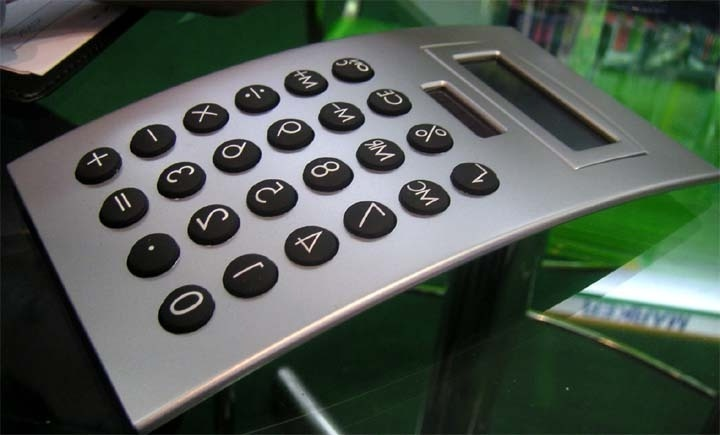
\includegraphics[width=0.8\linewidth]{pic/source.jpg}
                    \caption{Input}
                \end{figure}
            \end{column}
            \begin{column}{.5\linewidth}
                \begin{figure}
                    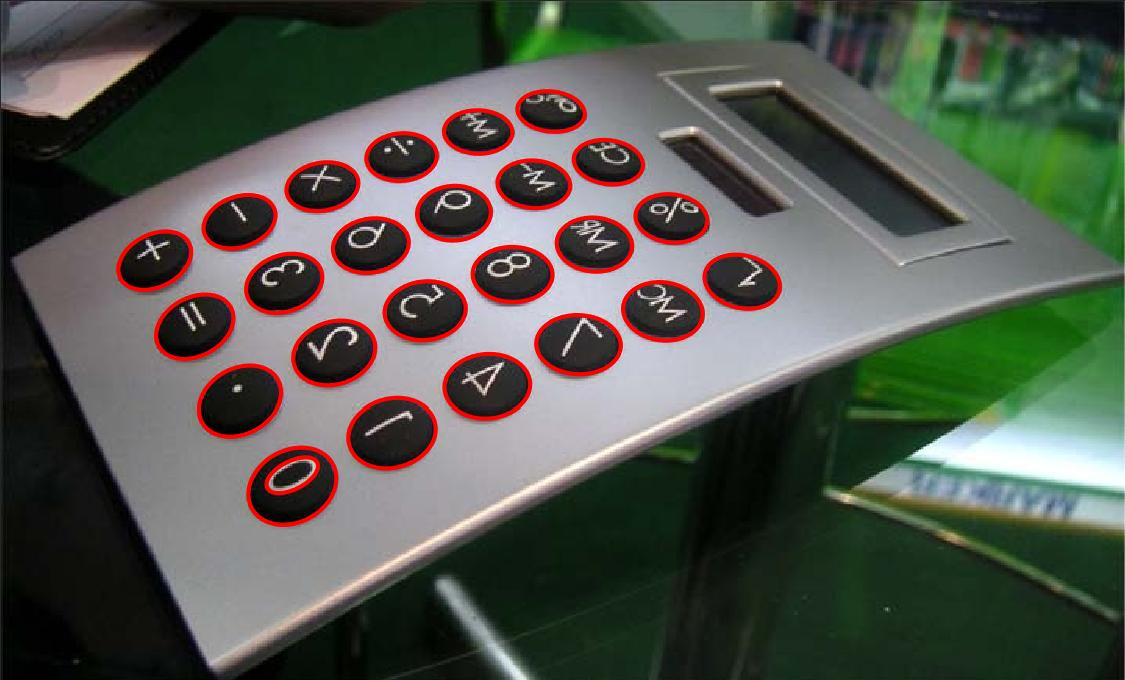
\includegraphics[width=0.8\linewidth]{pic/ideaoutput.jpg}
                    \caption{Output}
                \end{figure}
            \end{column}
        \end{columns}
    
    \end{frame}
    \section{Background}
    \subsection{Definition}
    \begin{frame}[allowframebreaks]
        \frametitle{Ellipse}

        To describe an ellipse we need 5 parameters:

        $$ Ax^2 + Bxy + Cy^2 + Dx + Ey + F = 0 , \text{where } B^2 - 4 AC < 0.$$

        Or in another way, we need the coordinates of the ellipse's center ($x_0, y_0$), semi-major/semi-minor axes ($a,b$),
        and a rotation angle ($\varphi$).
        \begin{figure}
            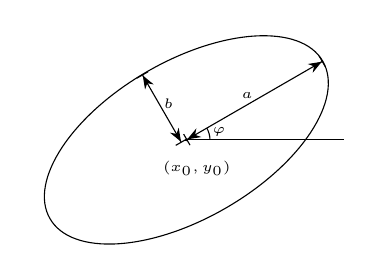
\begin{tikzpicture}
                \tikzstyle{every node}=[font=\tiny]
                \draw [rotate=30] (1,1) ellipse (2 and 1);
                \filldraw [rotate=30] (1,1) circle (.01);
                \draw [|{Stealth}-{Stealth}|,rotate=30,xshift =-2pt] (1,1)--(1,2);
                \draw [|{Stealth}-{Stealth}|,rotate=30] (1,1)--(3,1);
                \draw (0.5,1) node{$\left(x_0,y_0\right)$};
                \draw [xshift = 4pt,yshift = -2pt](0,1.9) node{$b$};
                \draw [xshift = 4pt,yshift = -2pt](1,2) node{$a$};
                \draw (0.366,1.366) -- (2.366,1.366 );
                \draw (0.666,1.366) arc (0:30:0.3);
                \draw (0.366,1.366) node[right,xshift = 6pt,yshift = 3pt]{$\varphi$};
                % \draw ({cos(75)} /{cos(45)} ,-1) -- ({cos(75)} /{cos(45)} ,1);
                % coordinate
                % \draw[->] (-3,0)--(3,0) node[right]{$x$};
                % \draw[->] (0,0)--(0,3) node[above]{$y$};
                % \draw[->,rotate = 30] (-3,0)--(3,0) node[right]{$x'$};
                % \draw[->,rotate = 30] (0,0)--(0,3) node[above]{$y'$};
                % \draw[->,rotate = 60] (-3,0)--(3,0) node[right]{$x''$};
                % \draw[->,rotate = 60] (0,0)--(0,3) node[above]{$y''$};
                % \draw [-,rotate=30] (1,1)--(-1,1);
            \end{tikzpicture}
            \caption{Parameters for the ellipse}
        \end{figure}
        

    \end{frame}
    \subsection{Related Work}
    \begin{frame}
        \frametitle{Two practical ways}
        
        

        \begin{columns}
            \begin{column}{.5\linewidth}
                Hough Transform
                \begin{itemize}
                    \item Slow
                    \item Sacrifice accuracy for efficiency
                \end{itemize}
            \end{column}
            \begin{column}{.5\linewidth}
                Edge Following
                \begin{itemize}
                    \item Derived from Arc-support LS 
                    \item use greyscale image (gradient)
                    \item Greedy for efficiency
                \end{itemize}
            \end{column}
        \end{columns}
        
    \end{frame}
    \section{Methods}
    \begin{frame}
        \frametitle{Methods}
    
        \begin{itemize}
            \item To detect the arc segments;
            \item (To form arcs;)
            \item To predict the 5 parameters for ellipses;
            \item Co-clustering;
            \item Validation.
        \end{itemize}
    
    \end{frame}
    \subsection{Arc segments}
    \begin{frame}
        \frametitle{LSD: A Fast Line Segment Detector with a False Detection Control}
        \framesubtitle{IEEE TRANSACTIONS ON PATTERN ANALYSIS AND MACHINE INTELLIGENCE}
        \begin{columns}
            \begin{column}{.5\linewidth}
                \begin{itemize}
                    \item Finding line-support region (region growing algorithm)
                    \item Rectangular Approximation of Regions
                    \item Validation
                \end{itemize}
                \begin{figure}
                    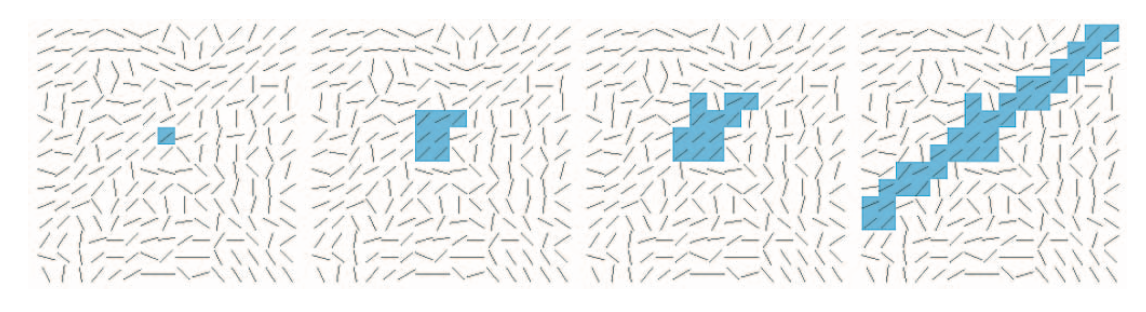
\includegraphics[width=\linewidth]{pic/region.png}
                    \caption{Region generation}
                \end{figure}
            \end{column}
            \begin{column}{.5\linewidth}
                
                \begin{figure}
                    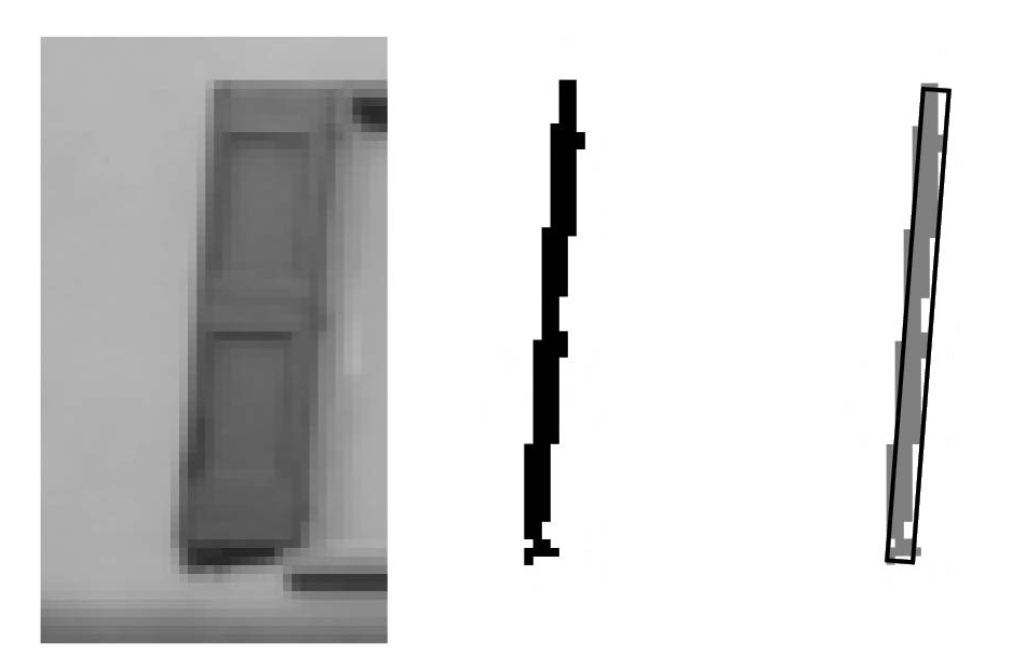
\includegraphics[width=.5\linewidth]{pic/rect.png}
                    \caption{Rectangular Approximation}
                \end{figure}
            \end{column}
        \end{columns}
    \end{frame}

    \begin{frame}
        \frametitle{Arc segments' result}
    
        \begin{columns}
            \begin{column}{.5\linewidth}
                \begin{figure}[htbp]
                    \centering
                    \subfigure{
                        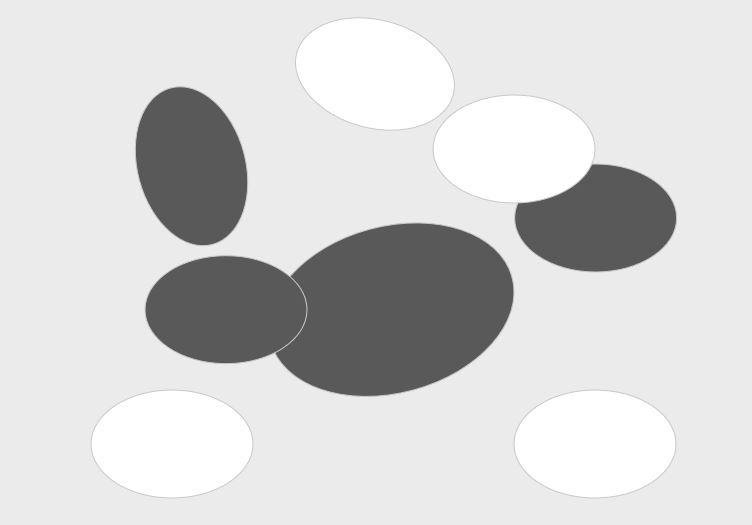
\includegraphics[width=0.7\linewidth]{pic/666.jpg}
                    }
                    \quad
                    \subfigure{
                        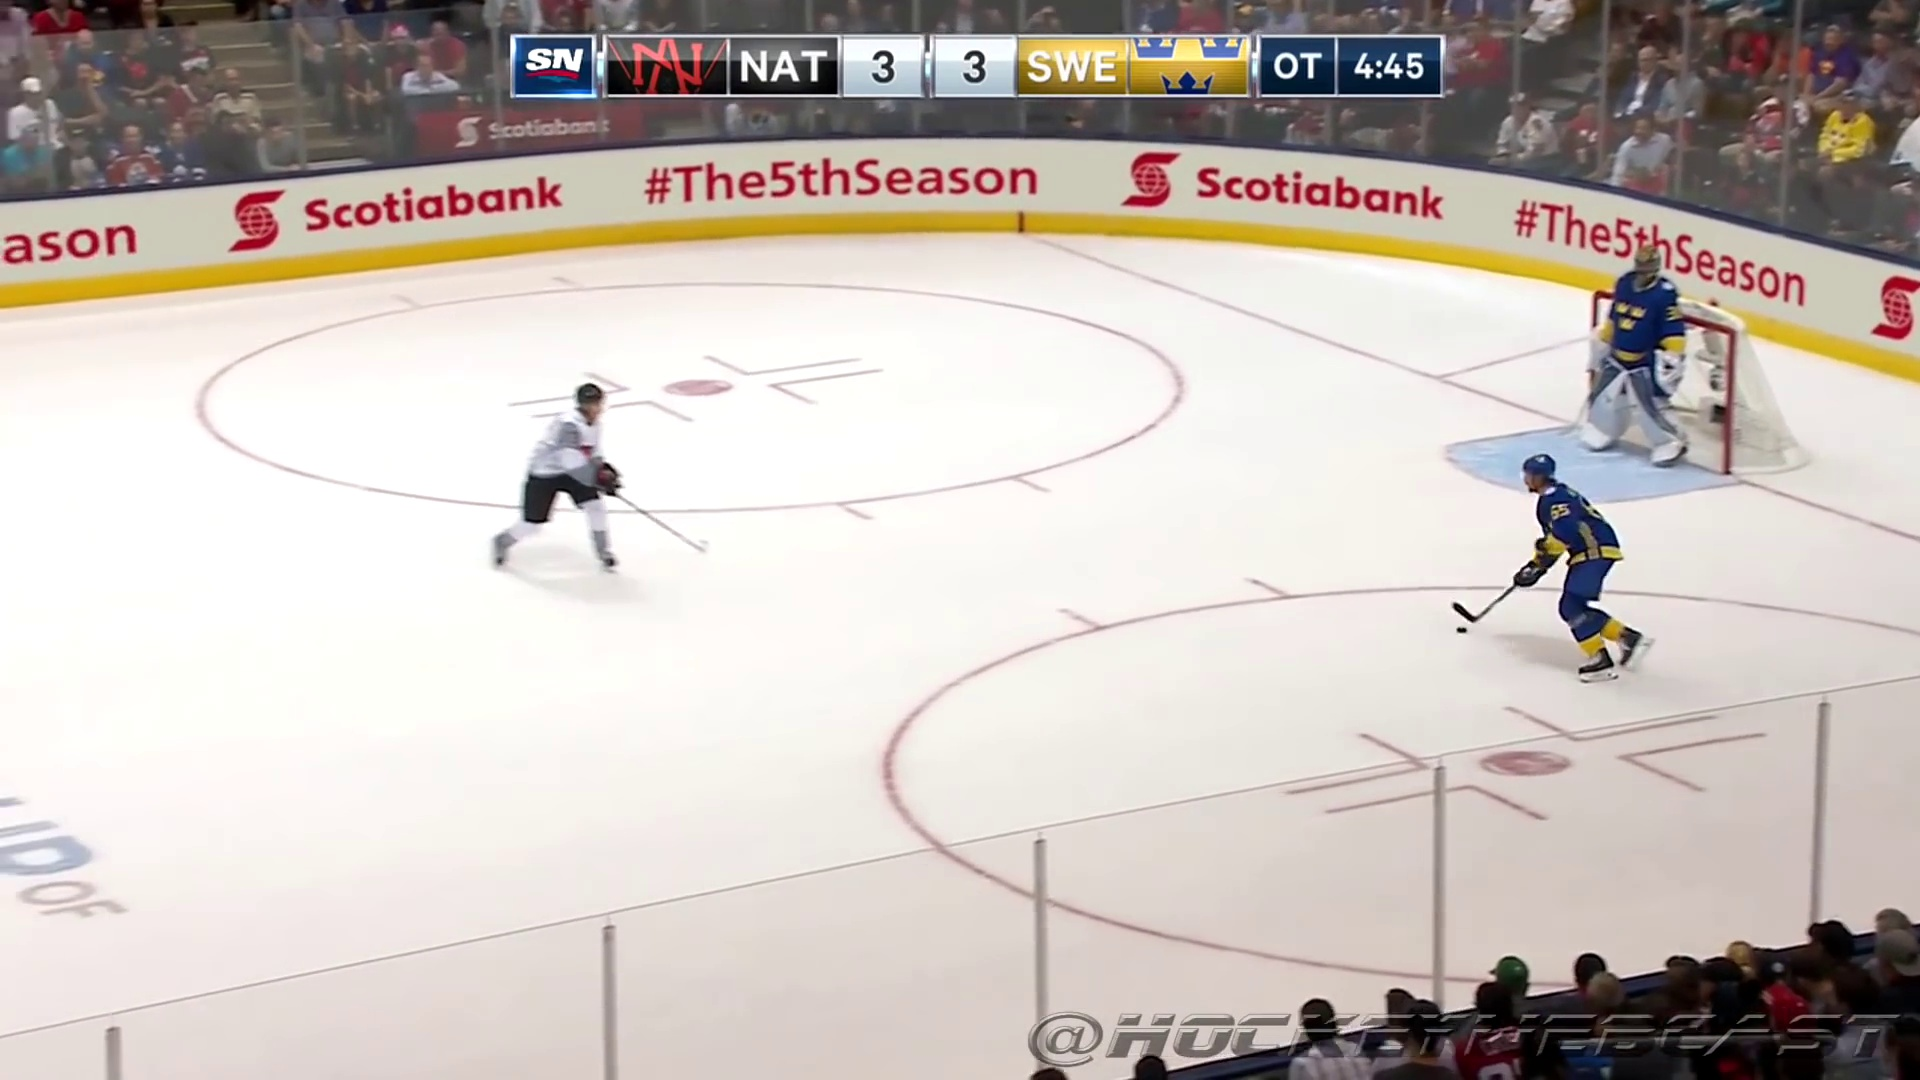
\includegraphics[width=0.7\linewidth]{pic/hockey.jpg}
                    }
                    \caption{Source Images}
                \end{figure}
            \end{column}
            \begin{column}{.5\linewidth}
                \begin{figure}[htbp]
                    \centering
                    \subfigure{
                        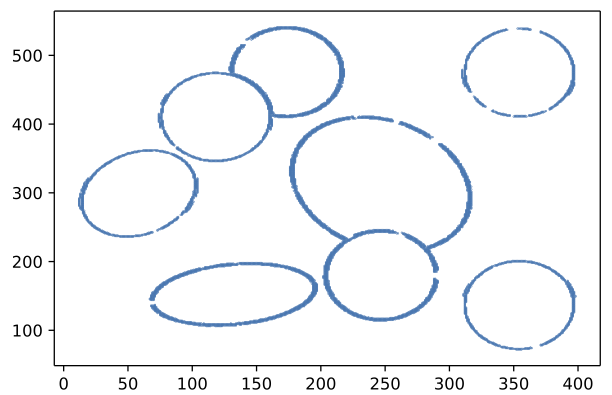
\includegraphics[width=0.7\linewidth]{pic/arc_666.png}
                    }
                    \quad
                    \subfigure{
                        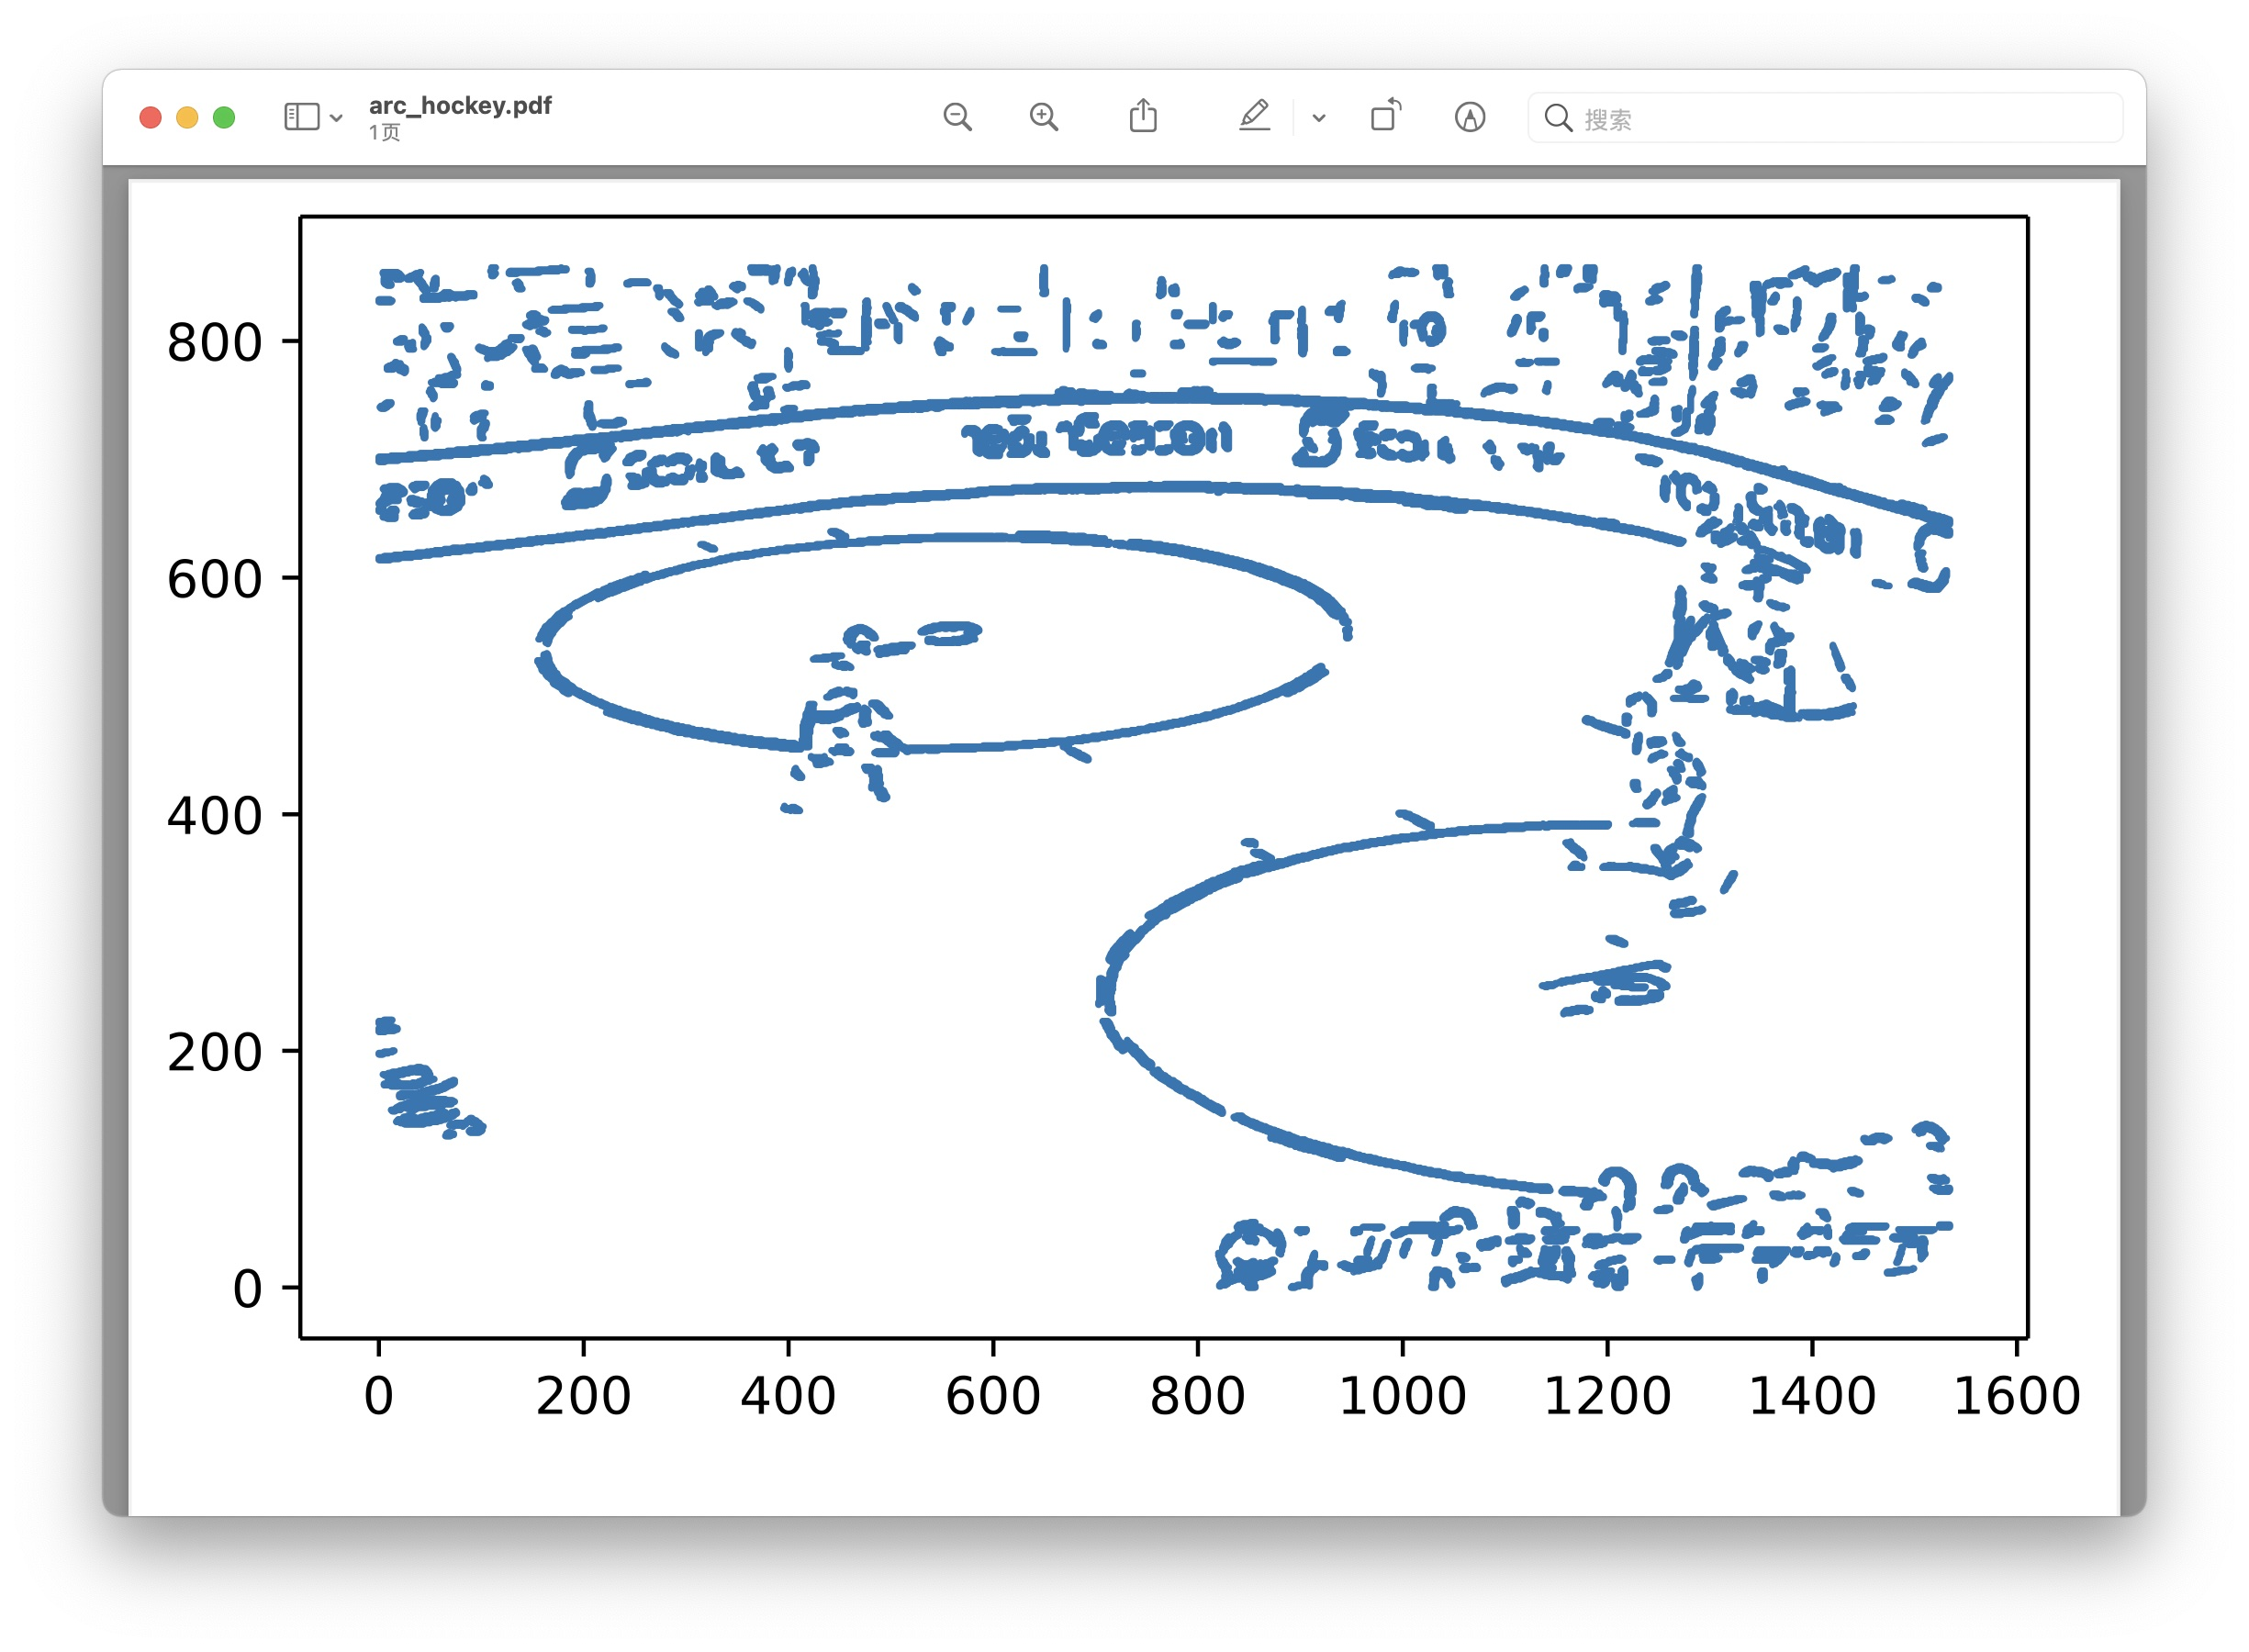
\includegraphics[width=0.7\linewidth]{pic/arc_hockey.jpg}
                    }
                    \caption{Arc Detection Results}
                \end{figure}
            \end{column}
        \end{columns}
    
    \end{frame}
    \subsection{Parameters Prediction}
    \begin{frame}
        \frametitle{Caluculating the Parameters}
    
        \begin{columns}
            \begin{column}
                {0.3\linewidth}
                \begin{figure}
                    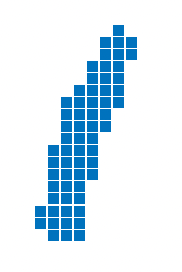
\includegraphics[width=\linewidth]{pic/arc.png}
                    \caption{Arc Segment Example}
                \end{figure}
            \end{column}
            
            \begin{column}{0.6\linewidth}
                \begin{onlyenv}<1>
                    $$x^2 + bxy +cy^2+dx+ey+f=0;$$
                    $$\begin{pmatrix}
                        x & y & 1
                    \end{pmatrix}
                    \begin{pmatrix}
                        1 & \frac{b}{2} & \frac{d}{2} \\
                        \frac{b}{2} & c & \frac{e}{2} \\
                        \frac{d}{2} & \frac{e}{2} & f
                    \end{pmatrix}
                    \begin{pmatrix}
                        x\\y\\1
                    \end{pmatrix} = O_{3\times3};$$
                    \begin{align*}
                        \begin{pmatrix}
                            x_1 & y_1 & 1 \\
                            \vdots & \vdots & \vdots \\
                            x_n & y_n & 1
                        \end{pmatrix}
                        \begin{pmatrix}
                            1 & \cfrac{b}{2} & \cfrac{d}{2} \\
                            \cfrac{b}{2} & c & \cfrac{e}{2} \\
                            \cfrac{d}{2} & \cfrac{e}{2} & f
                        \end{pmatrix}
                        \begin{pmatrix}
                            x_1 & \dots & x_n\\y_1 & \dots & y_n\\1 & \dots &1
                        \end{pmatrix} = O_{3\times3}.
                    \end{align*}
                \end{onlyenv}
                \begin{onlyenv}<2>
                    We can also alter it into:
                    \[\mathbf{D} \mathbf{\alpha} = \mathbf{0},\]
                    where \[
                        \mathbf{D} =
                        \begin{pmatrix}
                            _{1}^{2} & x_{1} y_{1} & y_{1}^{2} & x_{1} & y_{1} & 1 \\
                            x_{2}^{2} & x_{2} y_{2} & y_{2}^{2} & x_{2} & y_{2} & 1 \\
                            \vdots & \vdots & \vdots & \vdots & \vdots & \vdots \\
                            x_{n}^{2} & x_{n} y_{n} & y_{n}{ }^{2} & x_{n} & y_{n} & 1
                        \end{pmatrix};
                    \]
                    \[
                        \mathbf{\alpha}^{\mathbf{T}} = \begin{pmatrix}
                            1 & b & c & d &e & f
                        \end{pmatrix}
                    \]
                \end{onlyenv}
                
            \end{column}
        \end{columns}
        
    \end{frame}
    \subsection{cocluster}
    \begin{frame}[allowframebreaks]
        \frametitle{Cluster/Co-cocluster}
    
        After all the $\alpha_i$ ($i$ means the $i$th arc) are predicted,
        We correlate each two of them and then do co-clustering.

        Advantages of coclustering:
        \begin{enumerate}
            \item Fast for high-dimensional cluster jobs;
            \item Define co-distance in parameter space to represent the relativity.
        \end{enumerate}
        \framebreak

        \begin{figure}
            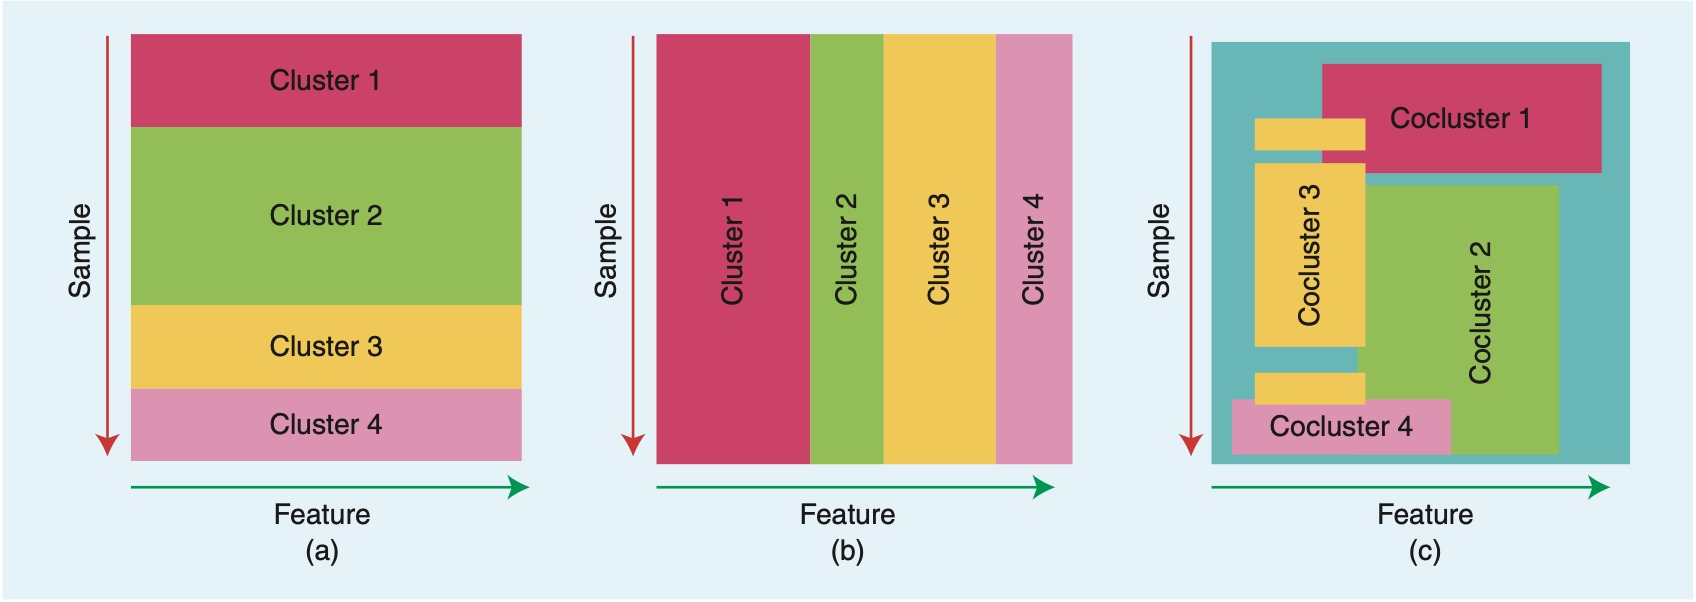
\includegraphics[width=0.8\linewidth]{pic/cocluster.png}
            \caption{cocluster method}
        \end{figure}
        \begin{figure}
            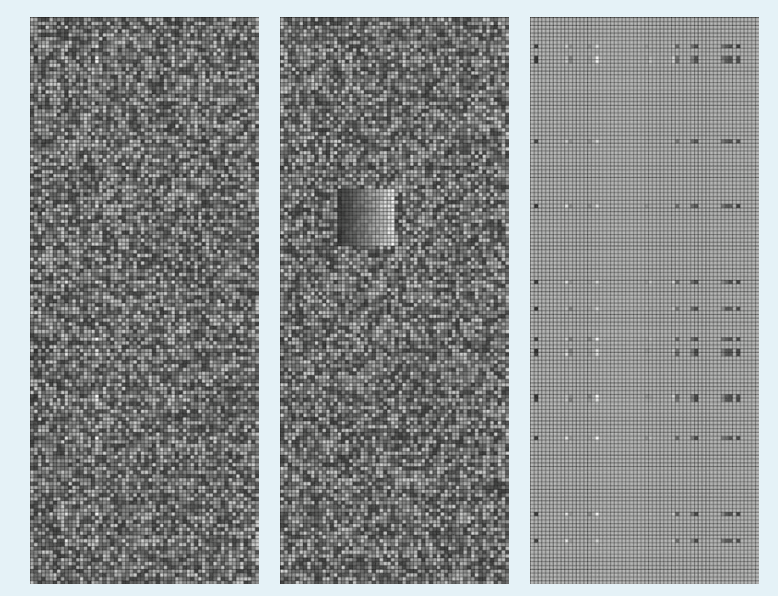
\includegraphics[width=0.5\linewidth]{pic/cocluster2.png}
            \caption{cocluster result}
        \end{figure}

    
    \end{frame}
    \subsection{Validation}
    \begin{frame}[allowframebreaks]
        \frametitle{Direct Least Square Fitting of Ellipses}
        \framesubtitle{PATTERN ANALYSIS AND MACHINE INTELLIGENCE}
        Lagrange multipliers
        $$
        \mathbf{D}=\left[\begin{array}{cccccc}
        x_{1}^{2} & x_{1} y_{1} & y_{1}^{2} & x_{1} & y_{1} & 1 \\
        x_{2}^{2} & x_{2} y_{2} & y_{2}^{2} & x_{2} & y_{2} & 1 \\
        \vdots & \vdots & \vdots & \vdots & \vdots & \vdots \\
        x_{n}^{2} & x_{n} y_{n} & y_{n}{ }^{2} & x_{n} & y_{n} & 1
        \end{array}\right]_{n \times 6}
        $$
        $$
        \mathbf{C}=\left[\begin{array}{ccccc}
        0 & 0 & -1 & \cdots & 0 \\
        0 & 2 & 0 & & \\
        -1 & 0 & 0 & & \vdots \\
        \vdots & & & \ddots & \\
        0 & & \cdots & & 0
        \end{array}\right]_{6 \times 6}
        $$

        \framebreak

        To minimize $||\mathrm{D} \mathrm{a}||^2$

        It turns into an optimization problem.
        $$
        \begin{array}{r}
        2 \mathrm{D}^{\mathrm{T}} \mathrm{D} \mathrm{a}-2 \lambda \mathrm{Ca}=0 \\
        \mathrm{a}^{T} \mathrm{Ca}=1
        \end{array}
        $$
    \end{frame}

    \begin{frame}
        \frametitle{Pilot Result}
        \begin{columns}
            \begin{column}{.5\linewidth}
                \begin{figure}[htbp]
                    \centering
                    \subfigure{
                        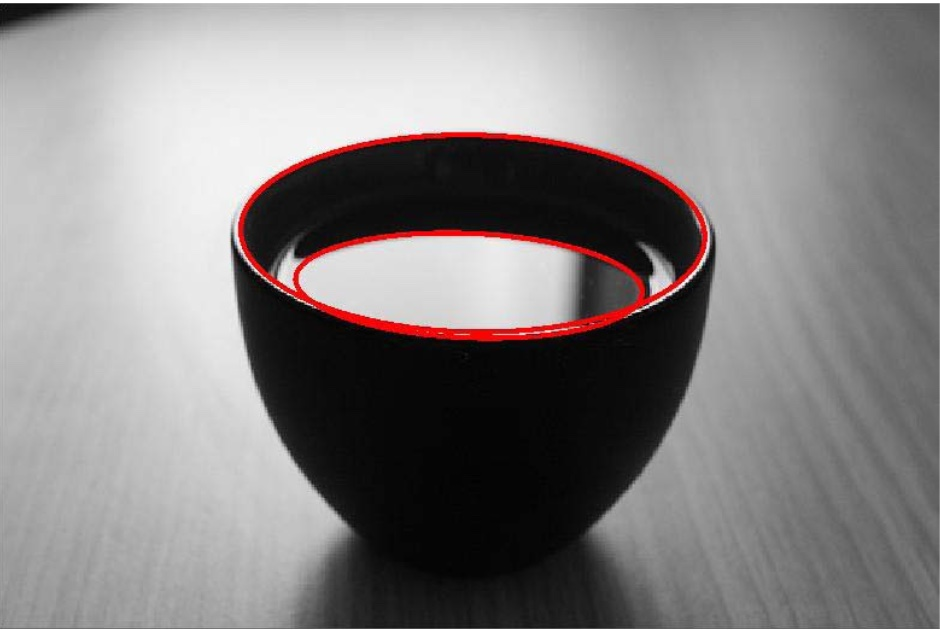
\includegraphics[width=0.7\linewidth]{pic/cup.jpg}
                    }
                    \quad
                    \subfigure{
                        \includegraphics[width=0.7\linewidth]{pic/coin.jpeg}
                    }
                    \caption{Good Examples}
                \end{figure}
            \end{column}
            \begin{column}{.5\linewidth}
                \begin{figure}[htbp]
                    \centering
                    \subfigure{
                        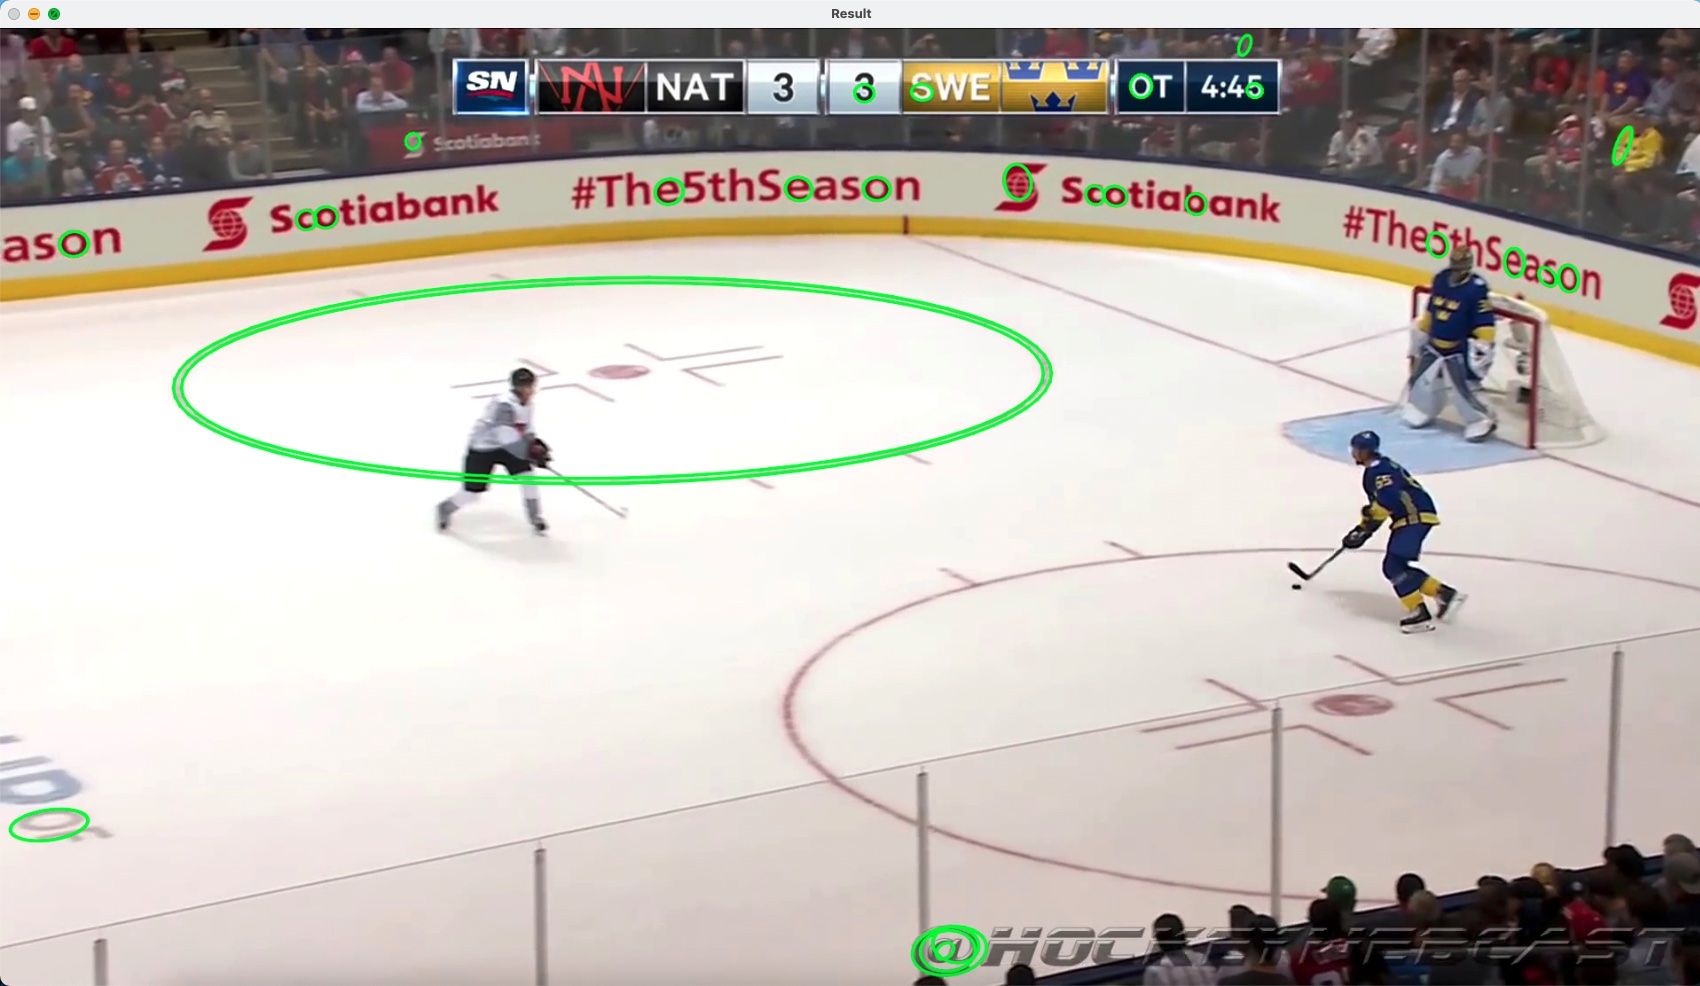
\includegraphics[width=0.7\linewidth]{pic/Hockeyre.jpg}
                    }
                    \quad
                    \subfigure{
                        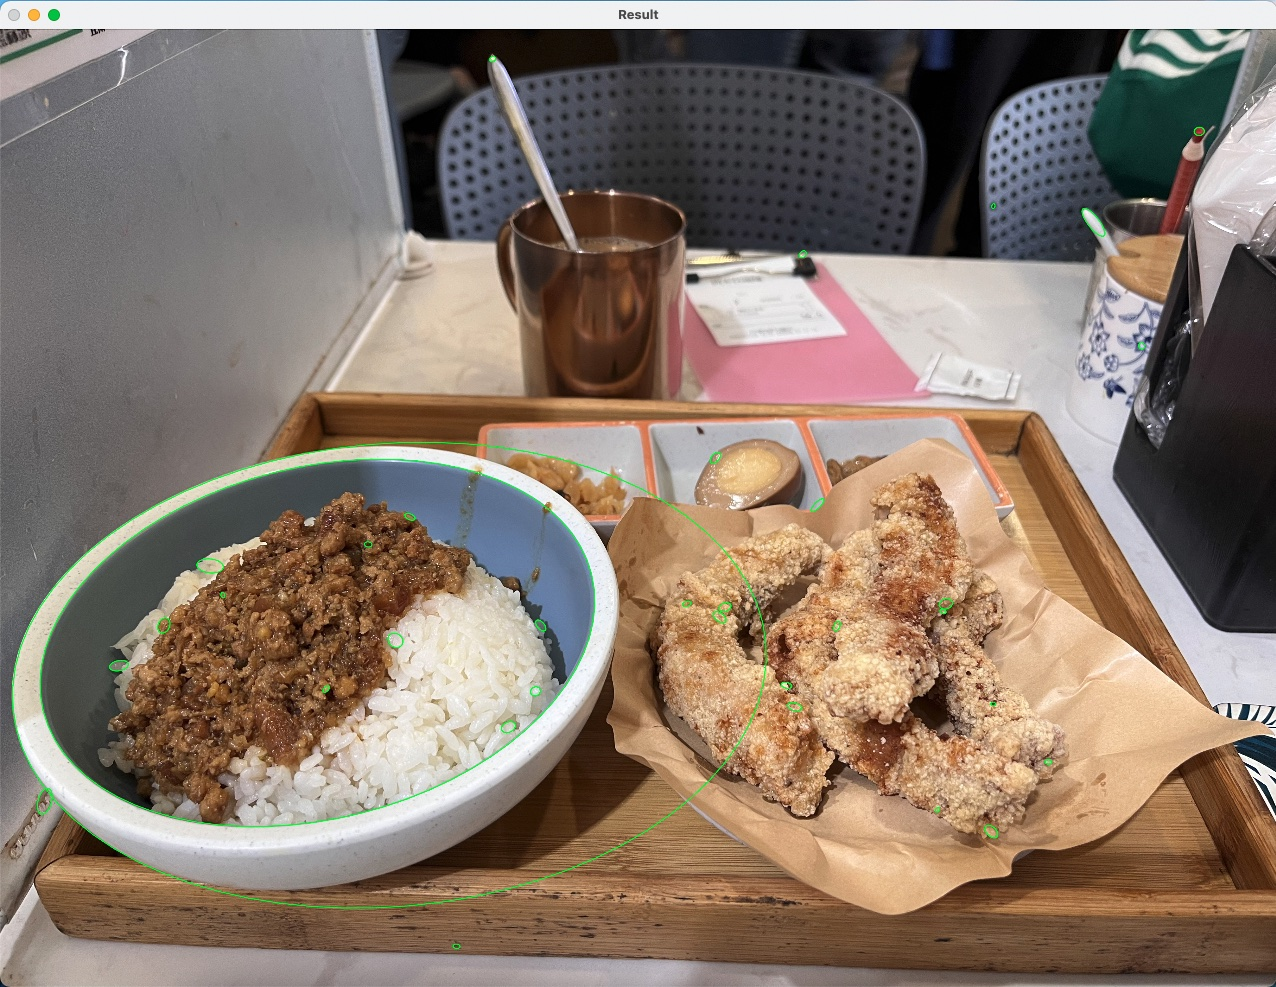
\includegraphics[width=0.7\linewidth]{pic/rice.jpg}
                    }
                    \caption{Bad Examples}
                \end{figure}
            \end{column}
        \end{columns}
        

    \end{frame}



    \begin{frame}
        \frametitle{Summary}
    
        \begin{enumerate}
            \item Co-clustering is effective in grouping data with good accuracy taking ellipses for example. 
            \item Co-clustering can serve as an unsupervised learning model in grouping problems.
            
        \end{enumerate}
    
    \end{frame}
    \begin{frame}
        \frametitle{Q\&A}
    
        Thank you!
    
    \end{frame}
\end{document}